\documentclass[11pt, oneside]{article}   	% use "amsart" instead of "article" for AMSLaTeX format
\usepackage{geometry}                		% See geometry.pdf to learn the layout options. There are lots.
\geometry{letterpaper}                   		% ... or a4paper or a5paper or ... 
%\geometry{landscape}                		% Activate for rotated page geometry
%\usepackage[parfill]{parskip}    		% Activate to begin paragraphs with an empty line rather than an indent
\usepackage{graphicx}				% Use pdf, png, jpg, or eps§ with pdflatex; use eps in DVI mode
								% TeX will automatically convert eps --> pdf in pdflatex		
\usepackage{float}
\usepackage{amssymb}


\usepackage{fancyhdr}
\usepackage{fancyhdr}
\fancyhead[L]{October 6, 2015}
\fancyhead[C]{SE 3XA3 Test Plan}
\fancyhead[R]{The A Team}
\pagestyle{fancy}


%SetFonts

%SetFonts


\title{Requirements Documentation}
\author{Gill, Surinder\\
		1308896
		\and
		Hu, Joshua\\
		1311940
		\and
		Lago, Nick\\
		1302613}
\date{October 6, 2015}							% Activate to display a given date or no date

%---------------------------------------------------------------------
\begin{document}
\maketitle
\newpage
%---------------------------------------------------------------------
\tableofcontents
\newpage
%---------------------------------------------------------------------

\section*{Revision History}

\begin{table}[hp]
\caption{Revision History: Proof of Concept Plan}
\begin{center}
\label{tab:}
\begin{tabular}{|c|c|c|c|}
\hline
\textbf{DATE} & \textbf{DEVELOPER} & \textbf{CHANGE} & \textbf{REVISION}\\
\hline
October 6, 2015 & Gill, Surinder & Initial Draft & 0\\
\hline
October 6, 2015 & Hu, Joshua & Initial Draft & 0\\
\hline
October 6, 2015 & Lago, Nick & Initial Draft & 0\\
\hline
\end{tabular}
\end{center}
\label{default}
\end{table}


\newpage
%---------------------------------------------------------------------
\section*{Project Drivers}
\subsection*{The Purpose of the Project}
\subsubsection*{The User Business or Background of the Project Effort}
This project is to re develop a popular game Flappy Bird and make it compatible with computers. Once the original developer Dong Nguyen took Flappy Bird off of app stores, the countless users no longer had means to download it. This meant that people would have to find similar games to fill the void that flappy bird left. With this product we will bring a similar game on a platform that is located in every household. Once completed anyone with a computer will be able to play the addicting and challenging game of flappy bird once again! Our motivation to make this project is to bring back one of the most popular app games in the interest of entertaining millions! This is not a serious problem but does provide a significant business opportunity for our clients. Flappy Bird at its highest point was making 50 000 dollars a day. By taking this game down there is a serious gap where fans of flappy bird are looking to find it elsewhere! Whether our client wishes to use this to gain profit off of people playing the game itself, or to gain extra traffic to their websites it is an opportunity that should not be overlooked! The completed project will be a JavaScript game similar to Flappy Bird to be played on web browsers. 


\subsubsection*{Goals of the Project}
Our product will be an entertainment driven experience for users who are interested in games that aren?t too complex but still contain challenging aspects. The goals for this project are creating a JavaScript game similar to Flappy Bird, documenting all processes involved in creation and getting a website to host our game. This way the client can have a working demonstration for the product we have designed and what their patrons will see when they access the product. The advantage to making this game in JavaScript is that this will make our game very website friendly. With this we can put the game on the internet for our clients to easily relay to their customers.  These are all service goals as they allow the user to access our product easier.


\subsection*{The Stakeholders}
\subsubsection*{The Client}
The client of our product is an external entity who is acting as the commissioner and final reviewer of our product prior to its deployment. They are an entity interested in redeploying the game "Flappy Bird" for the general public.


\subsubsection*{The Customer}
The customer of our project is the general public who will consume the game media. The archetypal customer would be a person with access to the internet and an interface which allows them to interact with the game, ergo an individual near the age of majority in a country with access to our product.


\subsubsection*{Other Stakeholders}
\begin{itemize}
\item Members of the public
\subitem These people will be our consumer base. They require no extraneous knowledge or background as the instructions for the product are basic and intuitive. In addition they require no involvement for the development of the project. As the project is a redevelopment of a previously existing product, the requirements that this stakeholder has been found through real market response and thus requires no further analysis.

\end{itemize}


\subsubsection*{The Hands-On-Users of the Product}
\begin{itemize}
\item University Students
\subitem Consumes media
\subitem Master consumer of media
\subitem Ability to access completed product
\subitem Opportunity to access and use product
\end{itemize}


\subsubsection*{Personas}
\begin{itemize}
\item Name: Abradolf Lincoler
\subitem Age: 38
\subitem Job: Unemployed
\subitem Family: Rick Sanchez, Father
\subitem Hobbies: Debating moral philosophy
\subitem City: Kirkjub\ae jarklaustur, Iceland
\subitem Favourite Food: Turkey feet
\subitem Favourite Music: Post Nu-Grunge Revival
\subitem Likes: Birds, Fish, Flappy things, Floppy things
\subitem Dislikes Requirements Documentation
\subitem Holiday Destination:  Hamilton, ON, Canada
\subitem Attitude to Technology: Mildly Positive
\subitem Attitude to Money: Indifferent
\end{itemize}


\subsubsection*{Priorities Assigned to Users}

\textbf{Key Users:}\\
The Client\\
The Customer\\
\\
\textbf{Secondary Users:}\\
The General Public\\
\\
\textbf{Unimportant Users:}\\
The General Public\\


\subsubsection*{User Participation}
\textbf{The Client:}\\
No input necessary.\\
\\
\textbf{The Customer}\\
No input necessary.\\
\\
\textbf{The General Public:}\\
No input necessary.\\


\subsubsection*{Maintenance Users and Service Technicians}
\textbf{Project Maintenance Team}\\
These users will maintain the relevance of code in the project and the performance of the website and servers.


\newpage
%---------------------------------------------------------------------
\section*{Project Constraints}
\subsection*{Mandated Constraints}
\subsubsection*{Solution Constraints}
Description: The product shall operate on browsers that allow JavaScript to run (i.e. computers, tablets, phones and other devices) through a website hosting server.
\\
\\
Rationale: The client will not be using outdated technology when accessing our website for our project. The client will be preferably using an up-to-date JavaScript client. 
\\
\\
Fit criterion: Our game client will be available to clients with browsers that have JavaScript and if it doesn?t, will prompt the user to go to the Java website. 
\\
\\
\\
Description: The product shall be played only when connected to the internet to load the game data and upload high scores. 
\\
\\
Rationale: The client should be connected to a secure internet connection with an upload and download speed that is appropriate to play the product. 
\\
\\
Fit criterion: The product shall be approved to play for users if they have a connection with a good enough internet speed that shall be determined with market research and our game requirements.
\\
\\
\\
Description: The product shall resize to different internet browsers and the different sizes/orientation that browsers use.
\\
\\
Rationale: The client would be able to resize their browser and the product shall resize accordingly until it hits a boundary where it cannot get any smaller or bigger.
\\
\\
Fit criterion: The product shall be able to resize to browsers on all devices and sizes where the game is able to be played. The maximum and minimum sizes will be determined through the game?s requirements and sprite sizes.

\subsubsection*{Implementation Environment of the Current System}
\begin{figure}[H] %  figure placement: here, top, bottom, or page
   \centering
   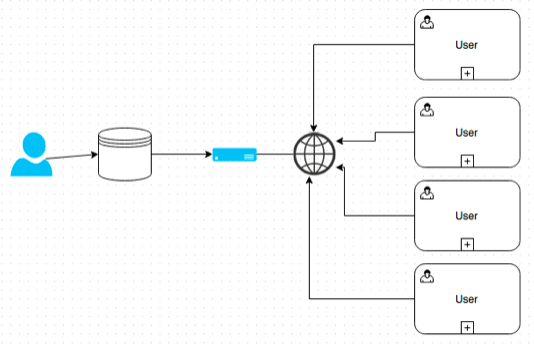
\includegraphics[width=6in]{ImplementationEnvironment.png} 
   \caption{Implementation Environment}
   \label{fig:example}
\end{figure}


\subsubsection*{Partner or Collaborative Applications}
The product does not have any direct partner or collaborative applications but does rely on text and picture editors to be created. It also relies on being able to run on a browser supporting JavaScript and if put out on market, a web-hosting server with a domain name.


\subsubsection*{Off-the-Shelf Software}
For the product to be executed the following off-the-shelf software is required:?\begin{itemize}
\item
A web browser (usually comes with the client)
\item
JavaScript (Available from https://java.com/en/download/)
\item
A client where the web browser can run (i.e. phone, tablet, computer, etc.)
\end{itemize}

All three of the OTS software can be received for free off the Internet as it is open-source.


\subsubsection*{Anticipated Workspace Environment}
The anticipated workplace environment for the product is anywhere. It can be played in someone?s house in a permanent location. It can also be played on the go, whether that be on a laptop or mobile device. As long as there an internet or mobile data connection, the product can be used. It can be inaccessible for clients where they do not have service/internet connection.


\subsubsection*{Schedule Constraints}
The schedule constraints are not applicable to our company.  The window of opportunity would have been when Flappy Bird was taken down from the mobile market as people would be given a second chance to play the game. However, a deadline has been set to the beginning of December as a chance for our team to have a goal to reach for.


\subsubsection*{Budget Constraints}
The amount of the budget is not applicable to us. We are given all the resources to re-create a project and as a result, are not funding anything.


\subsubsection*{Enterprise Constraints}
This game will be free to play and accessible for any user that has access to a piece of technology that can access a browser. From the browser, they can direct themselves to our project and as long as they have JavaScript, they?ll be able to run the project.


\subsection*{Naming Conventions and Terminology}
\subsubsection*{Definitions of All Terms, Including Acronyms, Used by Stakeholders Involved in the Project}
\begin{table}[H]
\caption{Definitions}
\begin{center}
\begin{tabular}{|c|c|}
\hline
\hline
ACRONYM/ABBREVIATION & INTENDED MEANING\\
\hline
JS & JavaScript\\
\hline
HTML &Hypertext Markup Language\\
\hline
PHP & Hypertext Preprocessor\\
\hline
Ex & Example\\
\hline
OS & Operating System\\
\hline
ETC & Et Cetera\\
\hline
bool & A Boolean value\\
\hline
NaN & Not a Number\\
\hline
txt & Text file\\
\hline
git & Git lab\\
\hline
eng & engineer\\
\hline
TAT & The A Team\\
\hline
The A Team & Project Team\\
\hline
WTF & Write to File\\
\hline
DTF & Data Transfer Function\\
\hline
Product & The game that our company is developing\\
\hline
Project & The development of the product\\
\hline
Client & The group that the product is being developed for\\
\hline
Customer & Any individual or group that utilizes the product after completion\\
\hline
The program & The coding that makes up the game created\\
\hline
\hline
\end{tabular}
\end{center}
\label{default}
\end{table}%



\subsection*{Relevant Facts and Assumptions}
\subsubsection*{Relevant Facts}
Some relevant facts regarding this project are that there were 900 codes of line in the previous implementation of this game. The game has an MIT license and needs to be run through a server for other users to access the project.


\subsubsection*{Business Rules}
One business rule that we?ve created is that everyone should have the same of amount of work and should try to take initiative at certain areas where they feel stronger.


\subsubsection*{Assumptions}
Some assumptions that developers are making about the project is that all the text and photo editing software will be free and accessible for them, the web-hosting server will be free for launch and the written code will be encapsulated so that it won?t be taken and resold for monetary value. Since most electronic devices with Wi-Fi are able to connect to a browser, they?ll be able to reach a technological environment in which the product will operate.


\newpage
%---------------------------------------------------------------------
\section*{Functional Requirements}
\subsection*{The Scope of the Work}
\subsubsection*{The Current Situation}
\begin{figure}[H] %  figure placement: here, top, bottom, or page
   \centering
   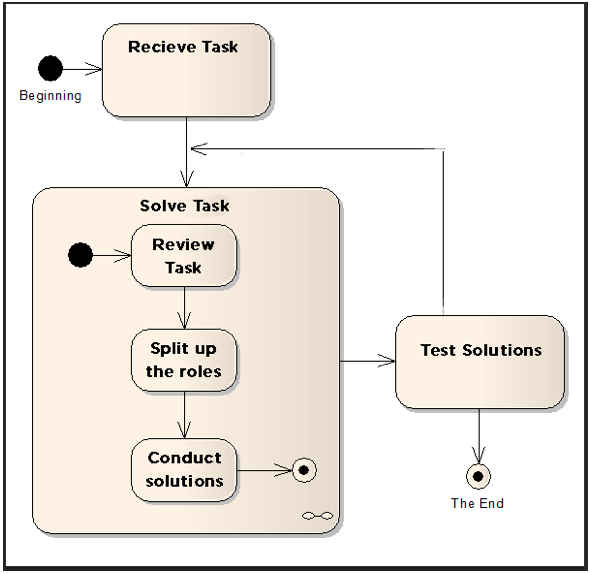
\includegraphics[width=6in]{ActivityDiagram.png} 
   \caption{Activity Diagram}
   \label{fig:example}
\end{figure}


\subsubsection*{The Context of the Work}
\begin{figure}[H] %  figure placement: here, top, bottom, or page
   \centering
   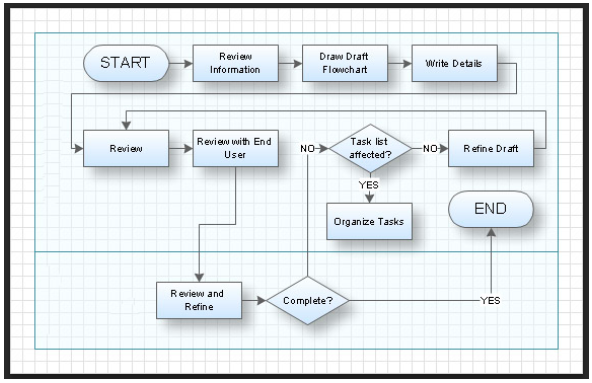
\includegraphics[width=6in]{Swimlane.png} 
   \caption{Swimlane Diagram}
   \label{fig:example}
\end{figure}


\subsubsection*{Work Partitioning}
\begin{table}[H]
\caption{Work Partitioning Part I}
\begin{center}
\begin{tabular}{|c|c|c|c|}
\hline
Event Number & Event Name & Input & Output\\
\hline
1 & Floppy Fish Creation & Developer code & Internet Browser\\
\hline
2 & Floppy Fish Audio & Microphone & Audio output device\\
\hline
3 & Floppy Fish Sprite & Developer graphics and code & Browser\\
\hline
4 & Floppy Fish Collisions & Developer code & Internet Browser\\
\hline
5 & Floppy Fish Final Edits & Developer code & Internet Browser\\
\hline
\end{tabular}
\end{center}
\label{default}
\end{table}%

\begin{table}[H]
\caption{Work Partitioning Part II}
\begin{center}
\begin{tabular}{|c|c|}

\hline
Event Number & Summary of BUC\\
\hline
1 & Recreate a browser based app that works on multiple\\ &different platforms and saves cookies on browsers\\
\hline
2 & Record and edit songs and sounds to be used in the project\\
\hline
3 & Create different functions of all the sprites and objects in the project\\
\hline
4 & Create collision detection and an end screen\\
\hline
5 & Finishing edits to the project\\
\hline

\end{tabular}
\end{center}
\label{default}
\end{table}%



\subsubsection*{Specifying a Business Use Case (BUC)}
Not applicable.


\subsection*{Business Data Model \& Data Dictionary}
\subsubsection*{Business Data Model}
\begin{figure}[H] %  figure placement: here, top, bottom, or page
   \centering
   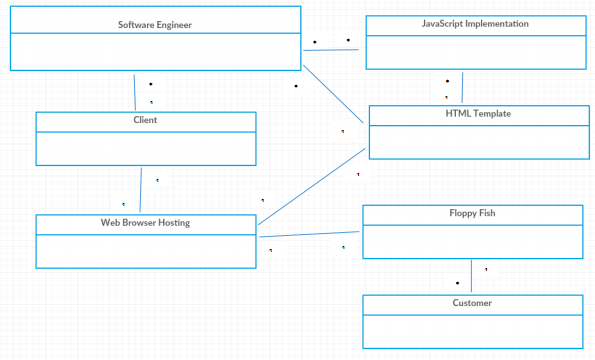
\includegraphics[width=6in]{BusinessDataModel.png} 
   \caption{Business Data Model}
   \label{fig:example}
\end{figure}

\subsubsection*{Data Dictionary}
\begin{table}[H]
\caption{Data Dictionary}
\begin{center}
\begin{tabular}{|c|c|c|}
\hline
Name & Content &Type\\
\hline
Software Engineer & engineerIdentifier & Class\\
\hline
Client & clientName	& Class\\
\hline
Web Browser Hosting & webBrowserIP + webBrowserDomain	& Class\\
\hline
Floppy Fish & floppyFishInstance & Class\\
\hline
JavaScript Implementation & isName + jsFunction & Class\\
\hline
HTML Template	 & templateName & Class\\
\hline
Customer	& Name + ID & Class\\
\hline
engineerIdentifier & *Unique Integer Identifier* & Attribute/ Element\\
\hline
ClientName & *String* & Attribute/ Element\\
\hline
webBrowserIP & *IP address* & Attribute/ Element\\
\hline
wedBrowserDomain & *Domain Address* & Attribute/ Element\\
\hline
floppyFishInstance & *Created Instance ID* & Attribute/ Element\\
\hline
jsName & *Document Name String*	& Attribute/ Element\\
\hline
jsFunction	& *Document Description String* & Attribute/ Element\\
\hline
templateName & *Naming String* & Attribute/ Element\\
\hline
\end{tabular}
\end{center}
\label{default}
\end{table}%



\subsection*{The Scope of the Product}
\subsubsection*{Project Boundary}



\subsubsection*{Product Use Case Table}



\subsubsection*{Individual Product Use Cases}



\subsection*{Functional Requirements}
\begin{itemize}
\item
The executable HTML file will create a new browser window.
\subitem
Fit Criterion or Test Case: \\
Is a new browser window created upon the execution of the HTML file?

\item
The HTML will be executed by a browser with JavaScript functionality.
\subitem
Fit Criterion or Test Case: \\
Attempt to execute the HTML file with multiple major browsers with HTML functionality.

\item
The game will have a standby state in which it waits for user input.
\subitem
Fit Criterion or Test Case: \\
Execute game and given an arbitrary timeframe if the game does not produces any unexpected action during that timeframe the game does not respond without user input.

\item
Upon the reception of user input from the standby state the game will begin.
\subitem
Fit Criterion or Test Case: \\
Provide user input to check if the state changes.

\item
At the beginning of the game the user will perceive all stats reset to their default state.
\subitem
Fit Criterion or Test Case: \\
Return the values of all stats upon the change from the default state.

\item
At the beginning of the game the user character will maintain its state until user input is received.
\subitem
Fit Criterion or Test Case: \\
Return relative character position at a regular interval prior to and during user input.

\item
If there is a collision with the user character and an obstacle object the game will terminate and all stats will be recorded.
\subitem
Fit Criterion or Test Case: \\
Given an arbitrary True value of a collision check see if the state changes and return the values of the stats.

\item
Upon termination of the game state all stats will be reset to their default state and the standby state will be reinitiated.
\subitem
Fit Criterion or Test Case: \\
Return the values of the stats and check the state.

\item
If there is a collision with the user character and an objective object the user's score will increment and the objective object's instance will terminate.
\subitem
Fit Criterion or Test Case: \\
Return the user's score, check the object's instance.

\item
During the game state reception of user input will cause the user character to respond in a constant and uniform manner relative to the user character's instance.
\subitem
Fit Criterion or Test Case: \\
Check the response of the user character.

\end{itemize}

\newpage
%---------------------------------------------------------------------
\section*{Non-functional Requirements}
\subsection*{Look and Feel Requirements}
\subsubsection*{Appearance Requirements}
The product shall display the logo of the client company upon starting. Floppy Fish will contain a vivid background of an ?underwater? scene. The product shall generate pipes of a solid colour from a predefined set of colours. Floppy Fish will contain a multicolored bright fish player to catch user?s eye while in gameplay. The background shall not overpower any colours of in game objects. The program will be sized to fit properly on a web page.


\subsubsection*{Style Requirements}
The product will generate pipes in a way that does not make the screen feel cluttered. Flappy Fish will appear to be a bright upbeat game. Flappy Fish shall have a retro style gameplay and fitting. Flappy Fish shall provide the user with a more intense feeling atmosphere rather than laid back. 


\subsection*{Usability and Humanity Requirements}
\subsubsection*{Ease of Use Requirements}
The game shall be able to be played by persons with appendages.


\subsubsection*{Personalization and Internationalization Requirements}
Not applicable.


\subsubsection*{Learning Requirements}
The user shall be able to operate an internet browser and a mouse.


\subsubsection*{Understandability and Politeness Requirements}
The user shall be able to operate an internet browser and a mouse.


\subsubsection*{Accessibility Requirements}
The game shall be able to be accessed and executed on the majority of user machines.


\subsection*{Performance Requirements}
\subsubsection*{Speed and Latency Requirements}
The game shall immediately by human perception respond to user input.


\subsubsection*{Safety-Critical Requirements}
The game shall not compromise the user data or machine.


\subsubsection*{Precision or Accuracy Requirements}
The game shall use integer values.


\subsubsection*{Reliability and Availability Requirements}
The game shall be available wherever there is an internet connection at any time when the servers are at or under maximum load.


\subsubsection*{Robustness or Fault-Tolerance Requirements}
The game shall be able to operate without consideration of the physical state of the end users.


\subsubsection*{Capacity Requirements}
The game shall not exceed the server load.


\subsubsection*{Scalability or Extensibility Requirements}
The code will allow for scalability.


\subsubsection*{Longevity Requirements}
The product shall be relevant for the lifetime of JavaScript functional browsers.


\subsection*{Operational and Environmental Requirements}
\subsubsection*{Expected Physical Environment}
The product is intended to be used anywhere there is a device that has a browser capabilities. The product shall be used in any environment that contains access to the internet.


\subsubsection*{Requirements for Interfacing with Adjacent Systems}
The product will be run on many different devices as long as the devices can open web browsers properly. The medium that will be carrying our interface is the website hosting our game.


\subsubsection*{Productization Requirements}
Before the product can be sold or distributed it must be hosted by a website for local use.

\subsubsection*{Release Requirements}
The product will be revised yearly and updated according to changing demands and needs of the client. The product will undergo maintenance upon realization of any errors in gameplay behaviour.


\subsection*{Maintainability and Support Requirements}
\subsubsection*{Maintenance Requirements}
Make maintenance of the product minimal.


\subsubsection*{Supportability Requirements}
Ensure the majority of potential users are capable of running the game on their machines.


\subsubsection*{Adaptability Requirements}
The game shall be universally acessable by users.


\subsection*{Security Requirements}
\subsubsection*{Access Requirements}
The entirety of the general public shall be able to access the game provided they have access to the necessary infrastructure.


\subsubsection*{Integrity Requirements}
The game shall not alter its source code.\\
The game shall not accept invalid user input.\\


\subsubsection*{Privacy Requirements}
The game shall not divulge data outside the game data.


\subsubsection*{Audit Requirements}
Not applicable.


\subsubsection*{Immunity Requirements}
Not applicable.


\subsection*{Cultural Requirements}
This product shall not be offensive to religious or ethnic groups. This product will be available in English. This product shall be hosted from the North American servers and accommodate ping from all over world.


\subsection*{Legal Requirements}
\subsubsection*{Compliance Requirements}
This game shall not compromise any laws.


\subsubsection*{Standards Requirements}
This game shall adhere to the MIT Open License.


\newpage
%---------------------------------------------------------------------
\section*{Project Issues}
\subsection*{Open Issues}
N/A


\subsection*{Off-the-shelf Solutions}
\subsubsection*{Ready-Made Products}
\begin{itemize}
\item Servers
\end{itemize}


\subsubsection*{Reusable Components}
Modularized code components.


\subsubsection*{Products That Can Be Copied}
As an open source project the original implementation can be relied upon as a prototype and source for code.


\subsection*{New Problems}
\subsubsection*{Effects on the Current Environment}
The new product will be one of hundreds of millions of different web addresses that host different products. It will not explode the Internet. However, if the server hosting is not able to hold all the users, then it can take down the server and other things being hosted by the server.


\subsubsection*{Effects on the Installed Systems}
This interface stands alone on and doesn?t coexist with an older system.


\subsubsection*{Potential User Problems}
Some potential user problems as an adverse reaction from playing our project are Carpel-tunnel syndrome and eye soreness/eye strain from extended playing.


\subsubsection*{Limitations in the Anticipated Implementation Environment That May Inhibit the New Product}
The server that will host our product will not be powerful enough to hold the desired amount of users with our project growth pattern.


\subsubsection*{Follow-Up Problems}
If we one of the developers leave the team, there will be a gap in the information for how the product is implemented. There are also adverse risks if the software becomes too outdated for new upcoming browsers and technology.


\subsection*{Tasks}
\subsubsection*{Project Planning}
\begin{table}[H]
\caption{default}
\begin{center}
\begin{tabular}{|c|c|c|}
\hline
Task	& Completer?s Role & Timeline\\
\hline
Model Implementation & Software Engineers & Oct 9th\\
\hline
Model Revision	& Client & Oct 10th\\
\hline
JavaScript design & Software Engineers & Oct 30th\\
\hline
HTML implementation & Software Engineers & Nov 3rd\\
\hline
Revision & Client & Nov 5th\\
\hline
Hosting & Software Engineers & Nov 23rd\\
\hline
Maintenance & Software Engineers & Yearly\\
\hline
\end{tabular}
\end{center}
\label{default}
\end{table}%



\subsubsection*{Planning of the Development Phases}
Phase 1 Model Implementation:
This phase is important as this will be the structure and backbone of our project. This is how we will set up the game and how each module interacts with each other. This should be operational before any coding is started. The product shall be based on this model.
Phase 2 Programming Implementation:
This phase is where we actually construct the program. Here we will create the game and test it. The program shall be run on JavaScript and HTML. The program will feel as if it is a Flappy Bird inspired game.
Phase 3 Hosting and Maintenance:
This phase requires us to put the game onto a server for people to play. At this point for optimal game experience the game shall be maintained at a high standard. This shall be completed and reviewed regularly or upon notice. The program will be continually playable throughout years to come. The program will remain functional as long as the client deems fit.


\subsection*{Migration to the New Product}
\subsubsection*{Requirements for Migration to the New Product}
None.


\subsubsection*{Data That Has to Be Modified or Translated for the New System}
None.


\subsection*{Risks}
None.


\subsection*{Costs}
None as long as the text and image editing software as well as web-hosting and domain name remain free.


\subsection*{User Documentation and Training}
\subsubsection*{User Documentation Requirements}
Not applicable.


\subsubsection*{Training Requirements}
Not applicable.


\subsection*{Waiting Room}
Additional functionality of the game functionality and visual as well as audio effects.


\subsection*{Ideas for Solutions}
Proper heirarchy and documentation of JavaScript code.


%---------------------------------------------------------------------
\end{document}  